\documentclass[12pt, letter]{article}
\usepackage{amsfonts}
\usepackage{amssymb}
\usepackage{amsthm}
\usepackage{amsmath}
\usepackage{graphicx}
\usepackage{multicol}
\usepackage{pifont}
\usepackage{multirow}

\hfuzz2pt % Don't bother to report over-full boxes if over-edge is < 2pt

\newcommand{\zag}[1]{\left(#1\right)}
\newcommand{\zagv}[1]{\left\{#1\right\}}
\newcommand{\zags}[1]{\left[#1\right]}
\def\ffrac#1/#2{\leavevmode\kern-.2em
  \raise.5ex\hbox{ $\textstyle #1$}\kern-.05em
  /\kern-.35em\lower.25ex\hbox{ $\textstyle #2$}}
\newcommand{\abs}[1]{\left\vert#1\right\vert}
\newcommand{\DS}{\displaystyle}
\newcommand{\SSS}{\scriptstyle}
\newcommand{\TS}{\textstyle}
\newcommand{\tg}{\mathrm{tg}\,}
\newcommand{\deo}[1]{\textbf{\textsf #1}}
\newcounter{zad}
\newcommand{\problem}[1]{{\setcounter{zad}{171}
\addtocounter{zad}{#1}\bigskip
\hskip -22pt\Huge{\ding{\value{zad}}}\hskip 0pt}}
\newcommand{\arctg}{\mathrm{arctg}\,}
\newcommand{\A}{\alpha}
\newcommand{\R}{\mathbb{R}}
\newcommand{\set}[1]{\left\{#1\right\}}
\newcommand{\slika}[1]{\
\vskip-0mm\includegraphics[width=3.5in]{#1}\vskip 5mm\ }
\newcommand{\slikav}[1]{\
\vskip-25mm \ \\
\begin{center}\includegraphics[width=175mm]{#1}\end{center}\vskip-10mm\ }
\newcommand{\tekst}[1]{\vfill #1 \vfill}
\newcommand{\opis}[2]{\small{\textbf{Figure.#1}\\ #2}}
\newenvironment{prob}{ }{\ }
\newcommand{\mat}[2][rrrrrrrrrrrrrrrrrrrrrrrrrrrrrrrrrrrrrr]{\left[
    \begin{array}{#1}
    #2\\
    \end{array}
    \right]}

\newcounter{zadatak}
\newcommand{\z}{\addtocounter{zadatak}{1} \hskip -14pt {{%
{\textbf{\arabic{zadatak}.}}}}\hskip 5pt}



\textheight 215mm \textwidth 155mm
\hoffset -10mm \voffset -20mm
\pagestyle{empty} \parindent 0pt \parskip 8pt

        
        
\begin{document}

 \begin{center}
 {\Large Estimating the evolution of scoring rates in soccer match: \\ Model selection and variable
 selection  with ???-LASSO}\\[1cm]
 {Mladen Laudanovic and Frank Wood}
 \end{center}
 

% % !TEX root = deplump.tex
\subsection*{Abstract}



%% !TEX root = main.tex
\section{Introduction}
\label{section_introduction}

Predictive models are all about doing as much as you can with as little data and computation as possible.  If sufficient for application purposes, resorting to simple models is often effective.  

Richly expressive models require   

Bayesian approaches to prediction dictate tying and sharing parameters, often through hierarchies and so forth. 

Cite 

Related work on multiscale language modeling
\citep{Goldwater2009,Mochihashi2009}

Related work on transformed Dirchlet processes and HDP's with random effects.
\citep{Sudderth2005,Kim2007,Hoffman2009,}

%\input{todo.tex}

\begin{equation*}
\begin{split}
\text{BASELINE MODEL 0:  }& y_{id}\mid X_{id}, \beta \sim \mathrm{Pois}\zag{\mu \alpha_{i}}\\
\text{BASELINE MODEL 1:  }& y_{id}\mid X_{id}, \beta \sim \mathrm{Pois}\zag{\lambda_{id}}\\
\text{BASELINE MODEL 2:  }& y_{id}\mid X_{id}, \beta \sim \mathrm{Pois}\zag{\alpha_{i}\lambda_{id}}\\
\text{BASELINE MODEL 3:  }& y_{id}\mid X_{id}, \beta \sim \mathrm{Pois}\zag{\mu \alpha_{i}}\\
\text{MODEL 1:  }& y_{id}\mid X_{id}, \beta \sim \mathrm{Pois}\zag{\lambda_{id}}\\
\text{MODEL 1':  }& y_{id}\mid X_{id}, \beta \sim \mathrm{Pois}\zag{\mu\lambda_{id}}\\
\text{MODEL 2:  }& y_{id}\mid X_{id}, \beta \sim \mathrm{Pois}\zag{\alpha_{i}\lambda_{id}}\\
\text{MODEL 2':  }& y_{id}\mid X_{id}, \beta \sim \mathrm{Pois}\zag{\mu\alpha_{i}\lambda_{id}}\\
\end{split}
\end{equation*}

where $\alpha_{i}$ are market intensities  and $\lambda_{id} = g(\beta^T X_{id})$ and also 
$$\text{MODEL 3':  } y_{id}\mid X_{id}, \beta \sim \mathrm{Pois}\zag{\alpha_{i}\lambda_{id}}$$
where $\alpha_{i}$ are unknown intensities. In this case likelihood is 
$$ \prod_i \prod_d \alpha_{i}^{y_{id}}\lambda_{id}^{y_{id}} e^{-\alpha_{i}\lambda_{id}}/y_{id}! = 
\prod_i \alpha_{i}^{\sum_d y_{id}} \prod_d \lambda_{id}^{y_{id}} e^{-\alpha_{i}\lambda_{id}}/y_{id}!$$ so $n_i = \sum_d y_{id}$ is sufficient statistic for $\alpha_i$, with the distribution $n_i \sim \mathrm{Pois}\zag{\alpha_{i}\sum_d\lambda_{id}}$. Likelihood for $n_i$ is  
$$ \prod_i \alpha_{i}^{n_{i}}\zag{\sum_d\lambda_{id}}^{n_{i}} e^{-\alpha_{i}\sum_d\lambda_{id}}/n_{i}! $$ hence after conditioning we get:
$$\text{MODEL 3:  } y_{i.}\mid \beta, n_i,  X_{i.}\sim \mathrm{M}
    \zag{n_i, \zagv{\frac{\lambda_{id}}{\sum_{d^\star}\lambda_{id^\star}}}_{d=1}^D}$$
 

   -- $d$ are minutes in a match (1-44, 46-89 for both teams; D = 176 per match)\\
   -- $i$ are matches ($I=302$)\\
   -- $g$ is a link function. There are three of them: $e^x, \log(1+e^x), \log(\frac{1}{1+e^{-x}})$\\
 
 Three models with three different link functions were tested. There were two subsets of variables, each one having 100 of them (selected by "quality", one without other with market variables)
 
   -- $K$ number of variables (K=100)

\newpage
MODEL1: $y_{id}\mid X_{id}, \beta \sim \mathrm{Pois}\zag{\lambda_{id}}$

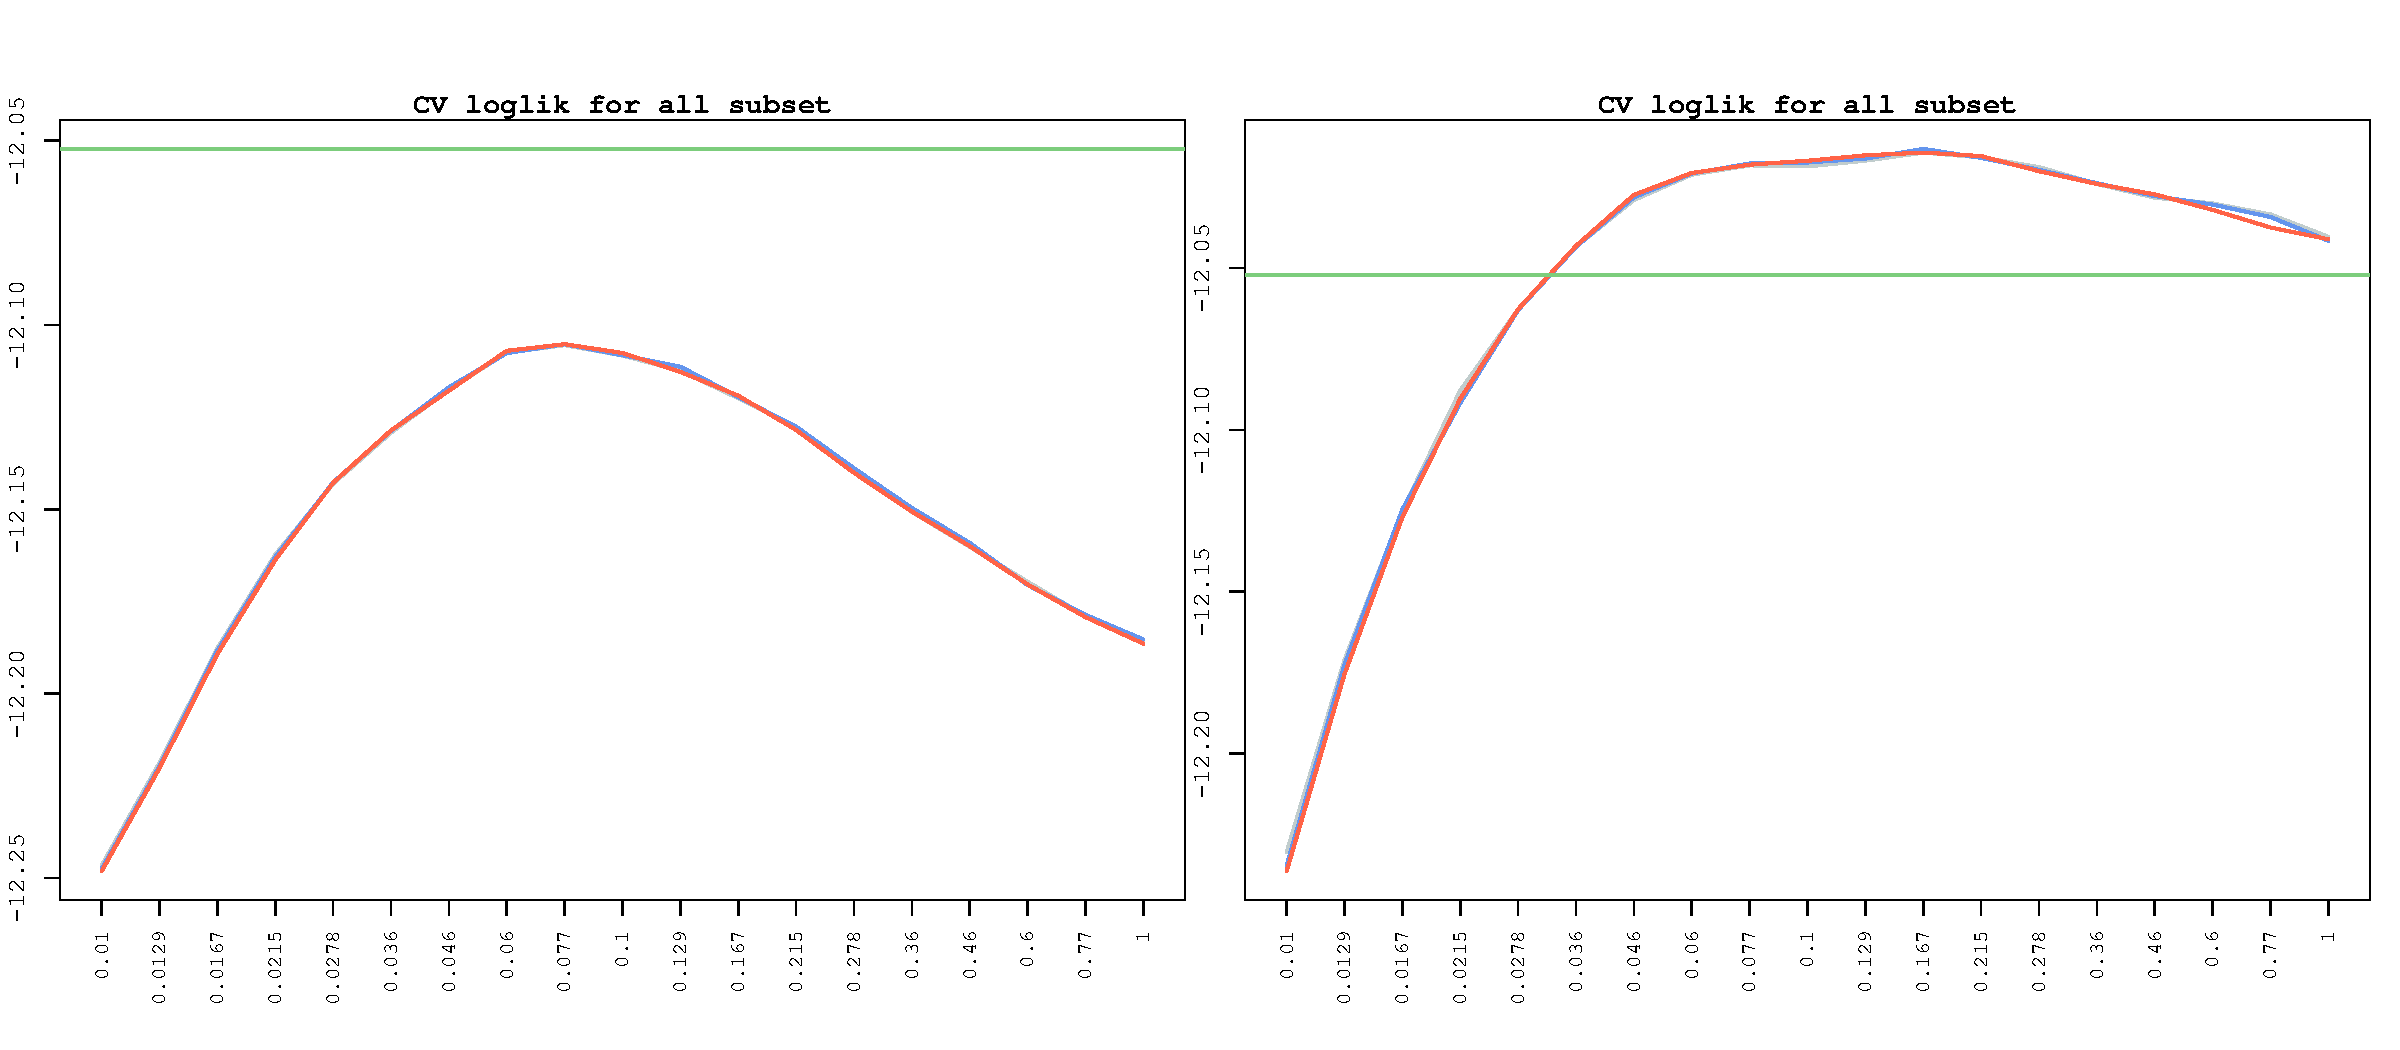
\includegraphics[width=6.5in]{basic.pdf}

%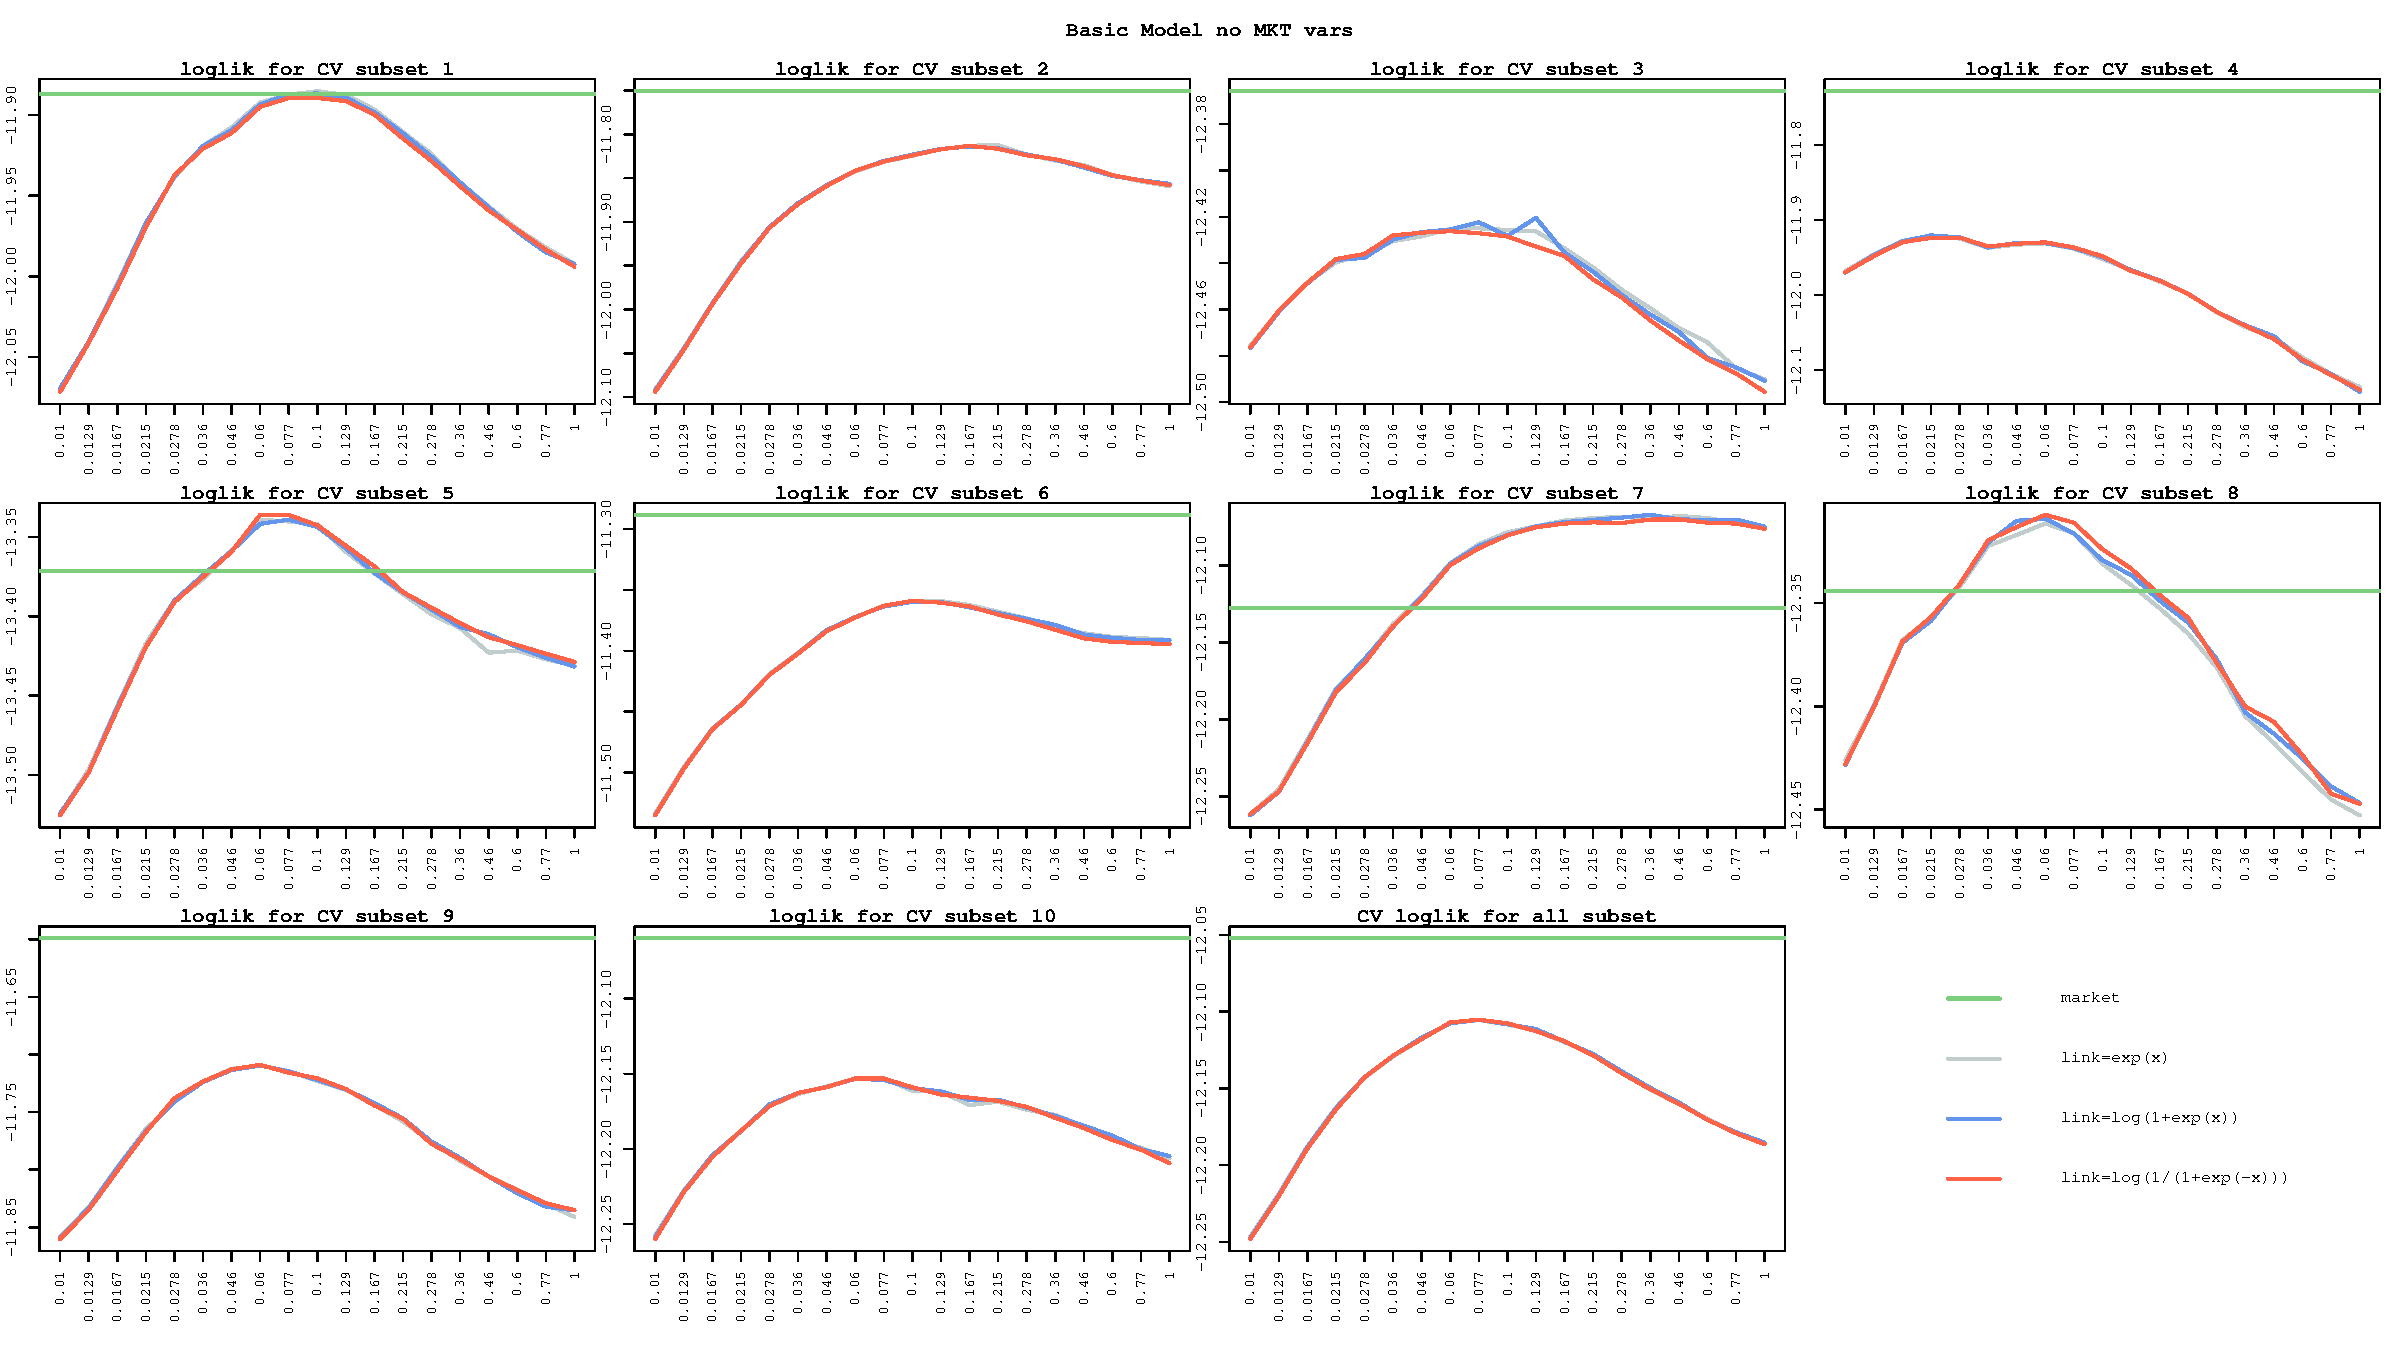
\includegraphics[width=6.5in]{compareBNM.pdf}
%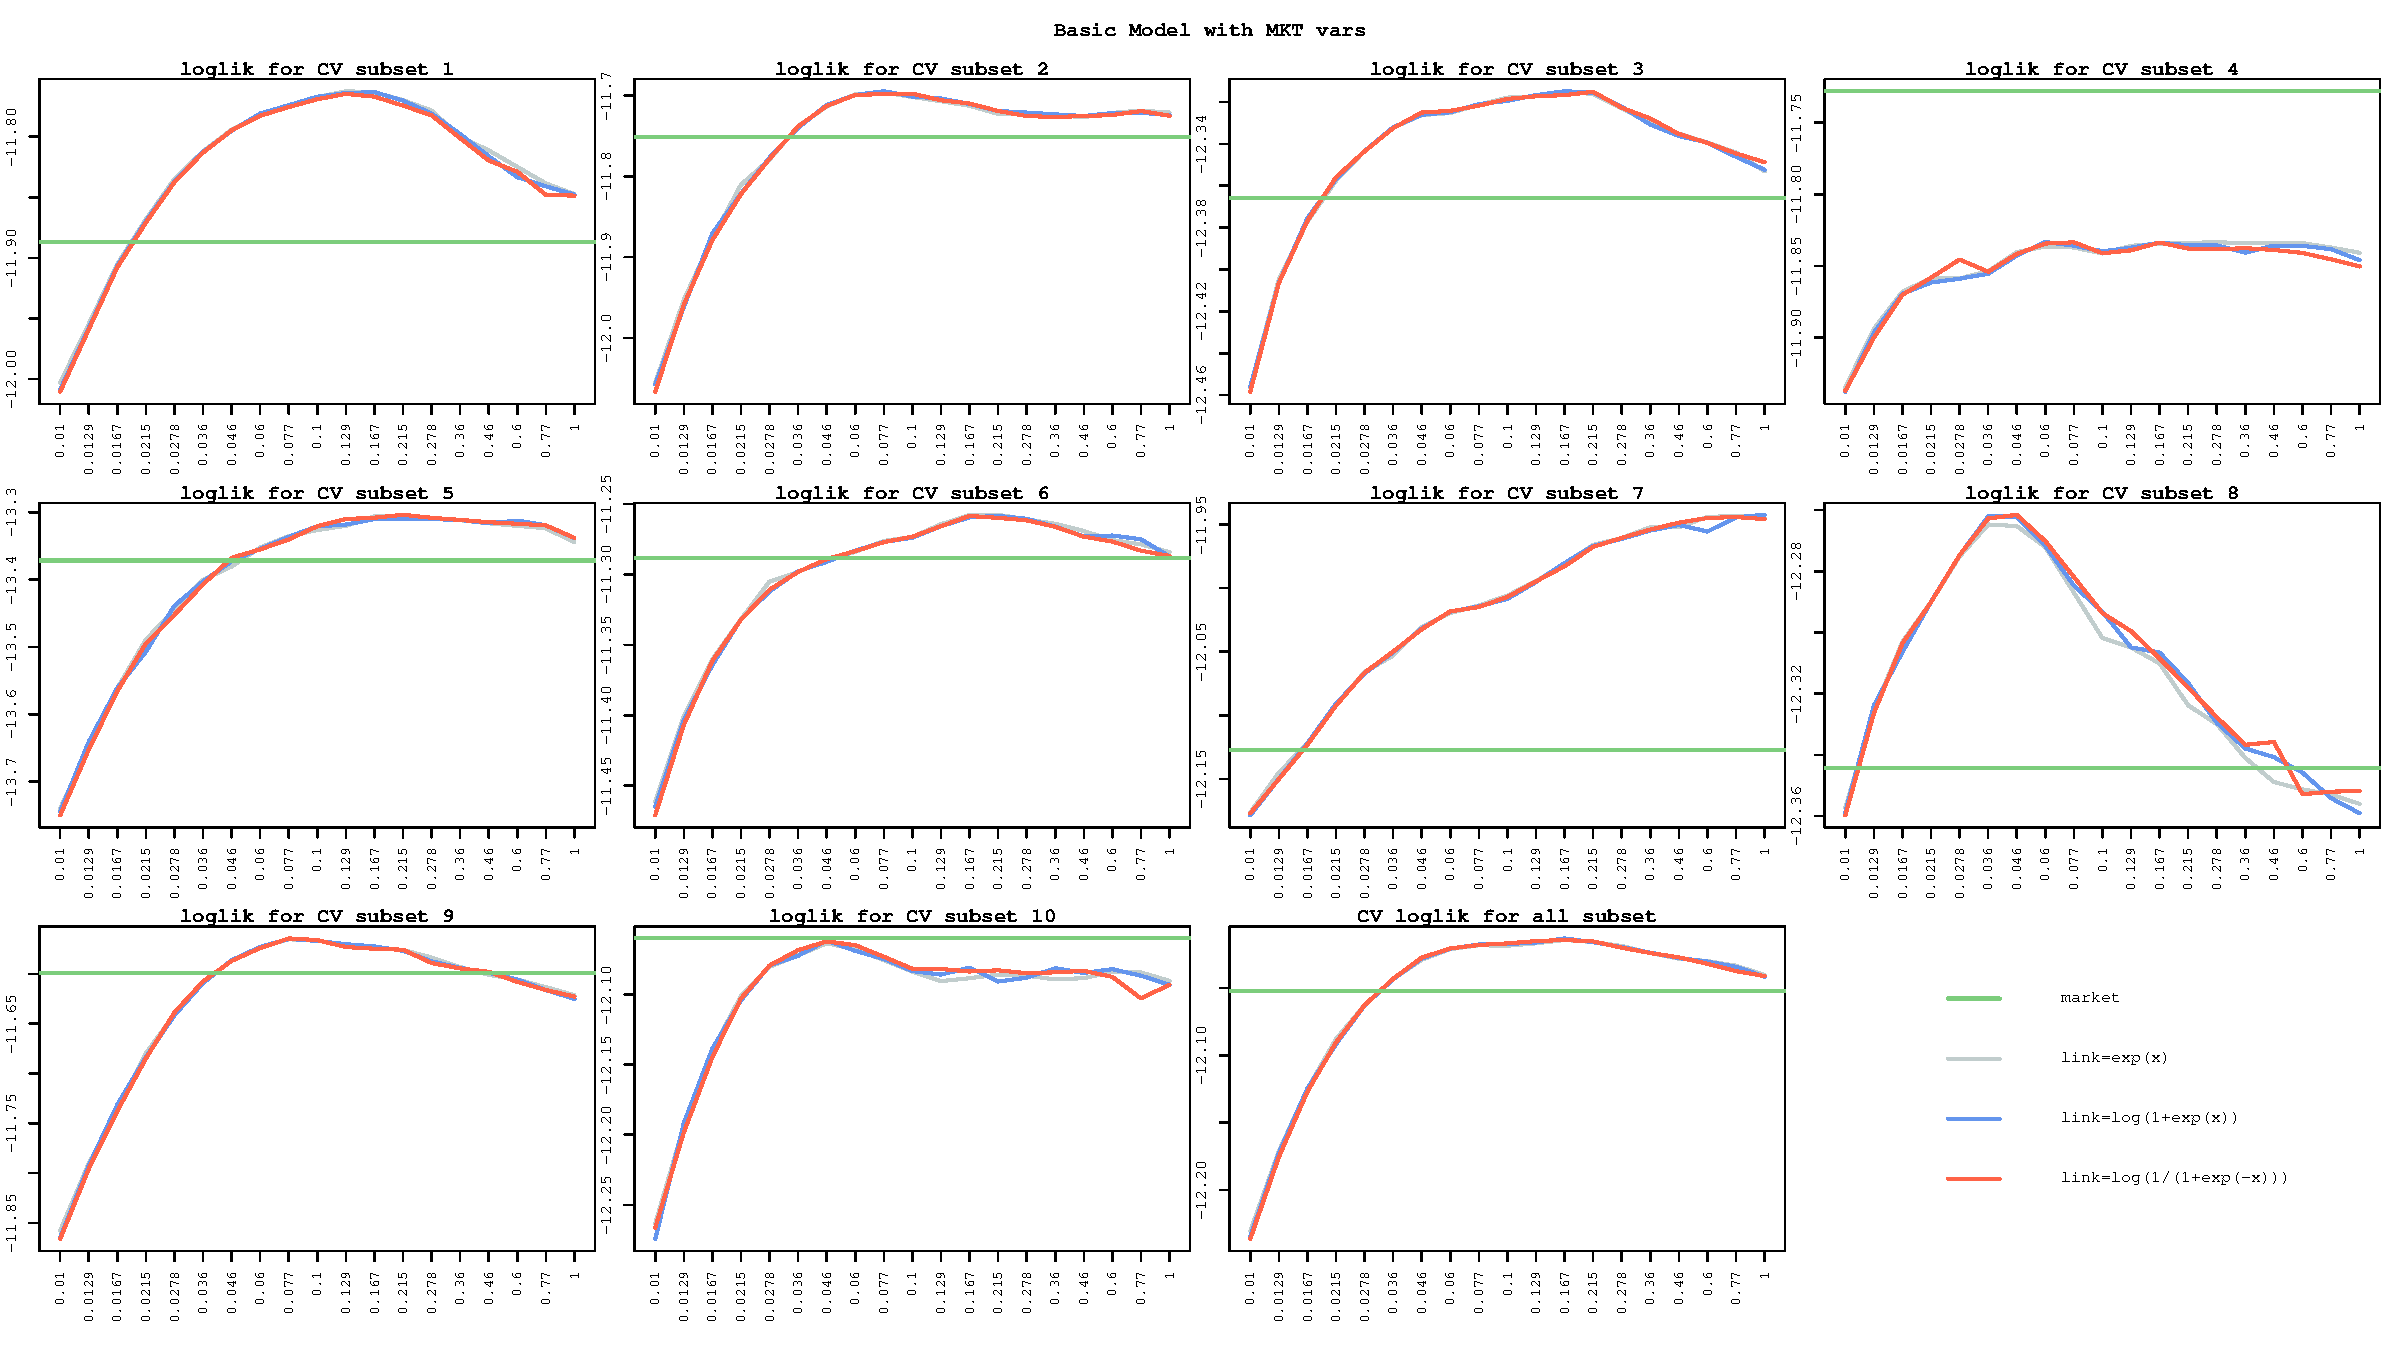
\includegraphics[width=6.5in]{compareBWM.pdf}
 
\newpage
MODEL2: $y_{id}\mid X_{id}, \beta \sim \mathrm{Pois}\zag{\alpha_{i}\lambda_{id}}$

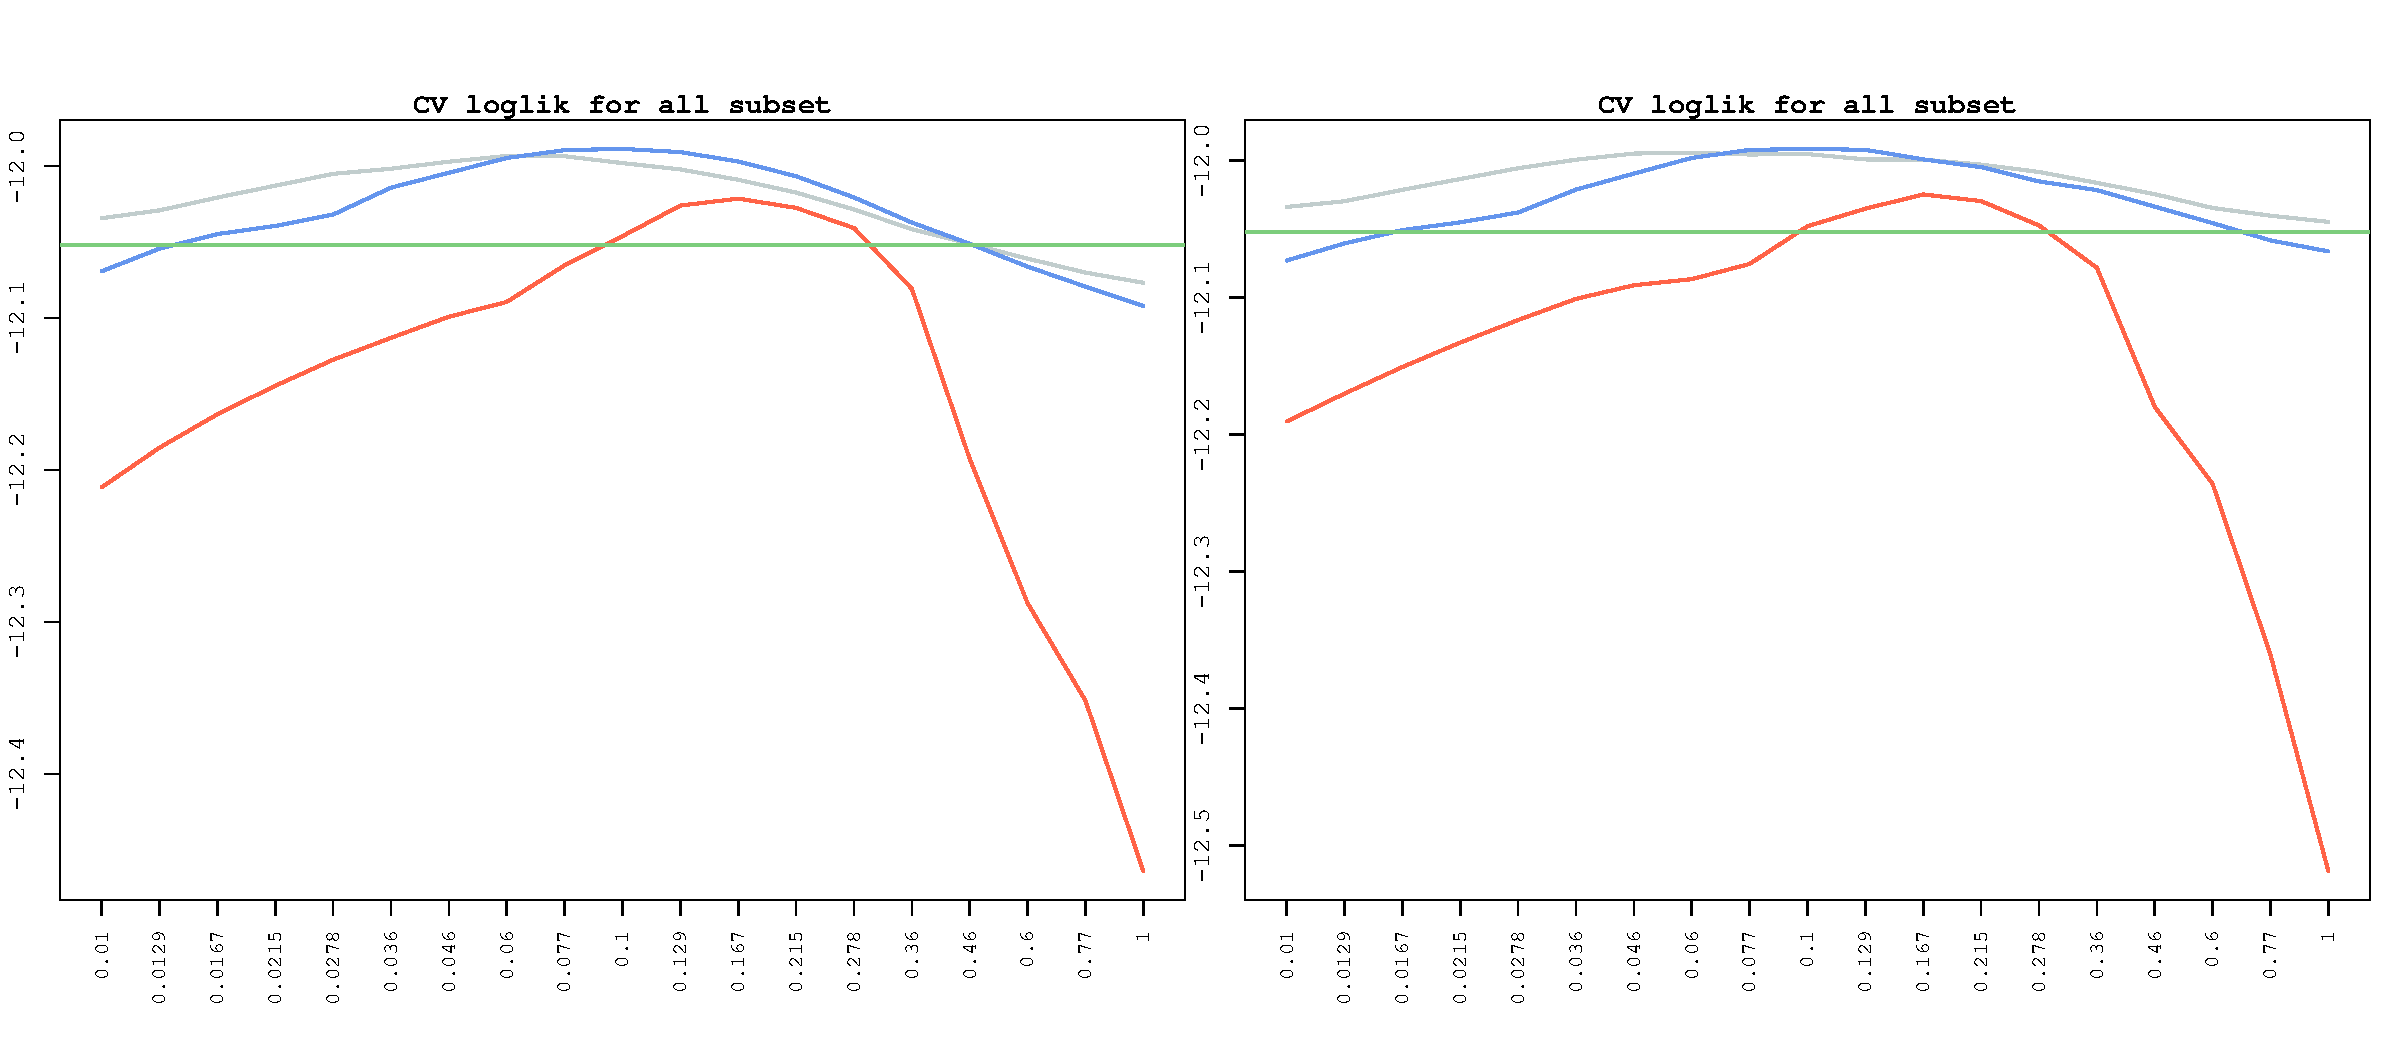
\includegraphics[width=6.5in]{basicMKT.pdf}


%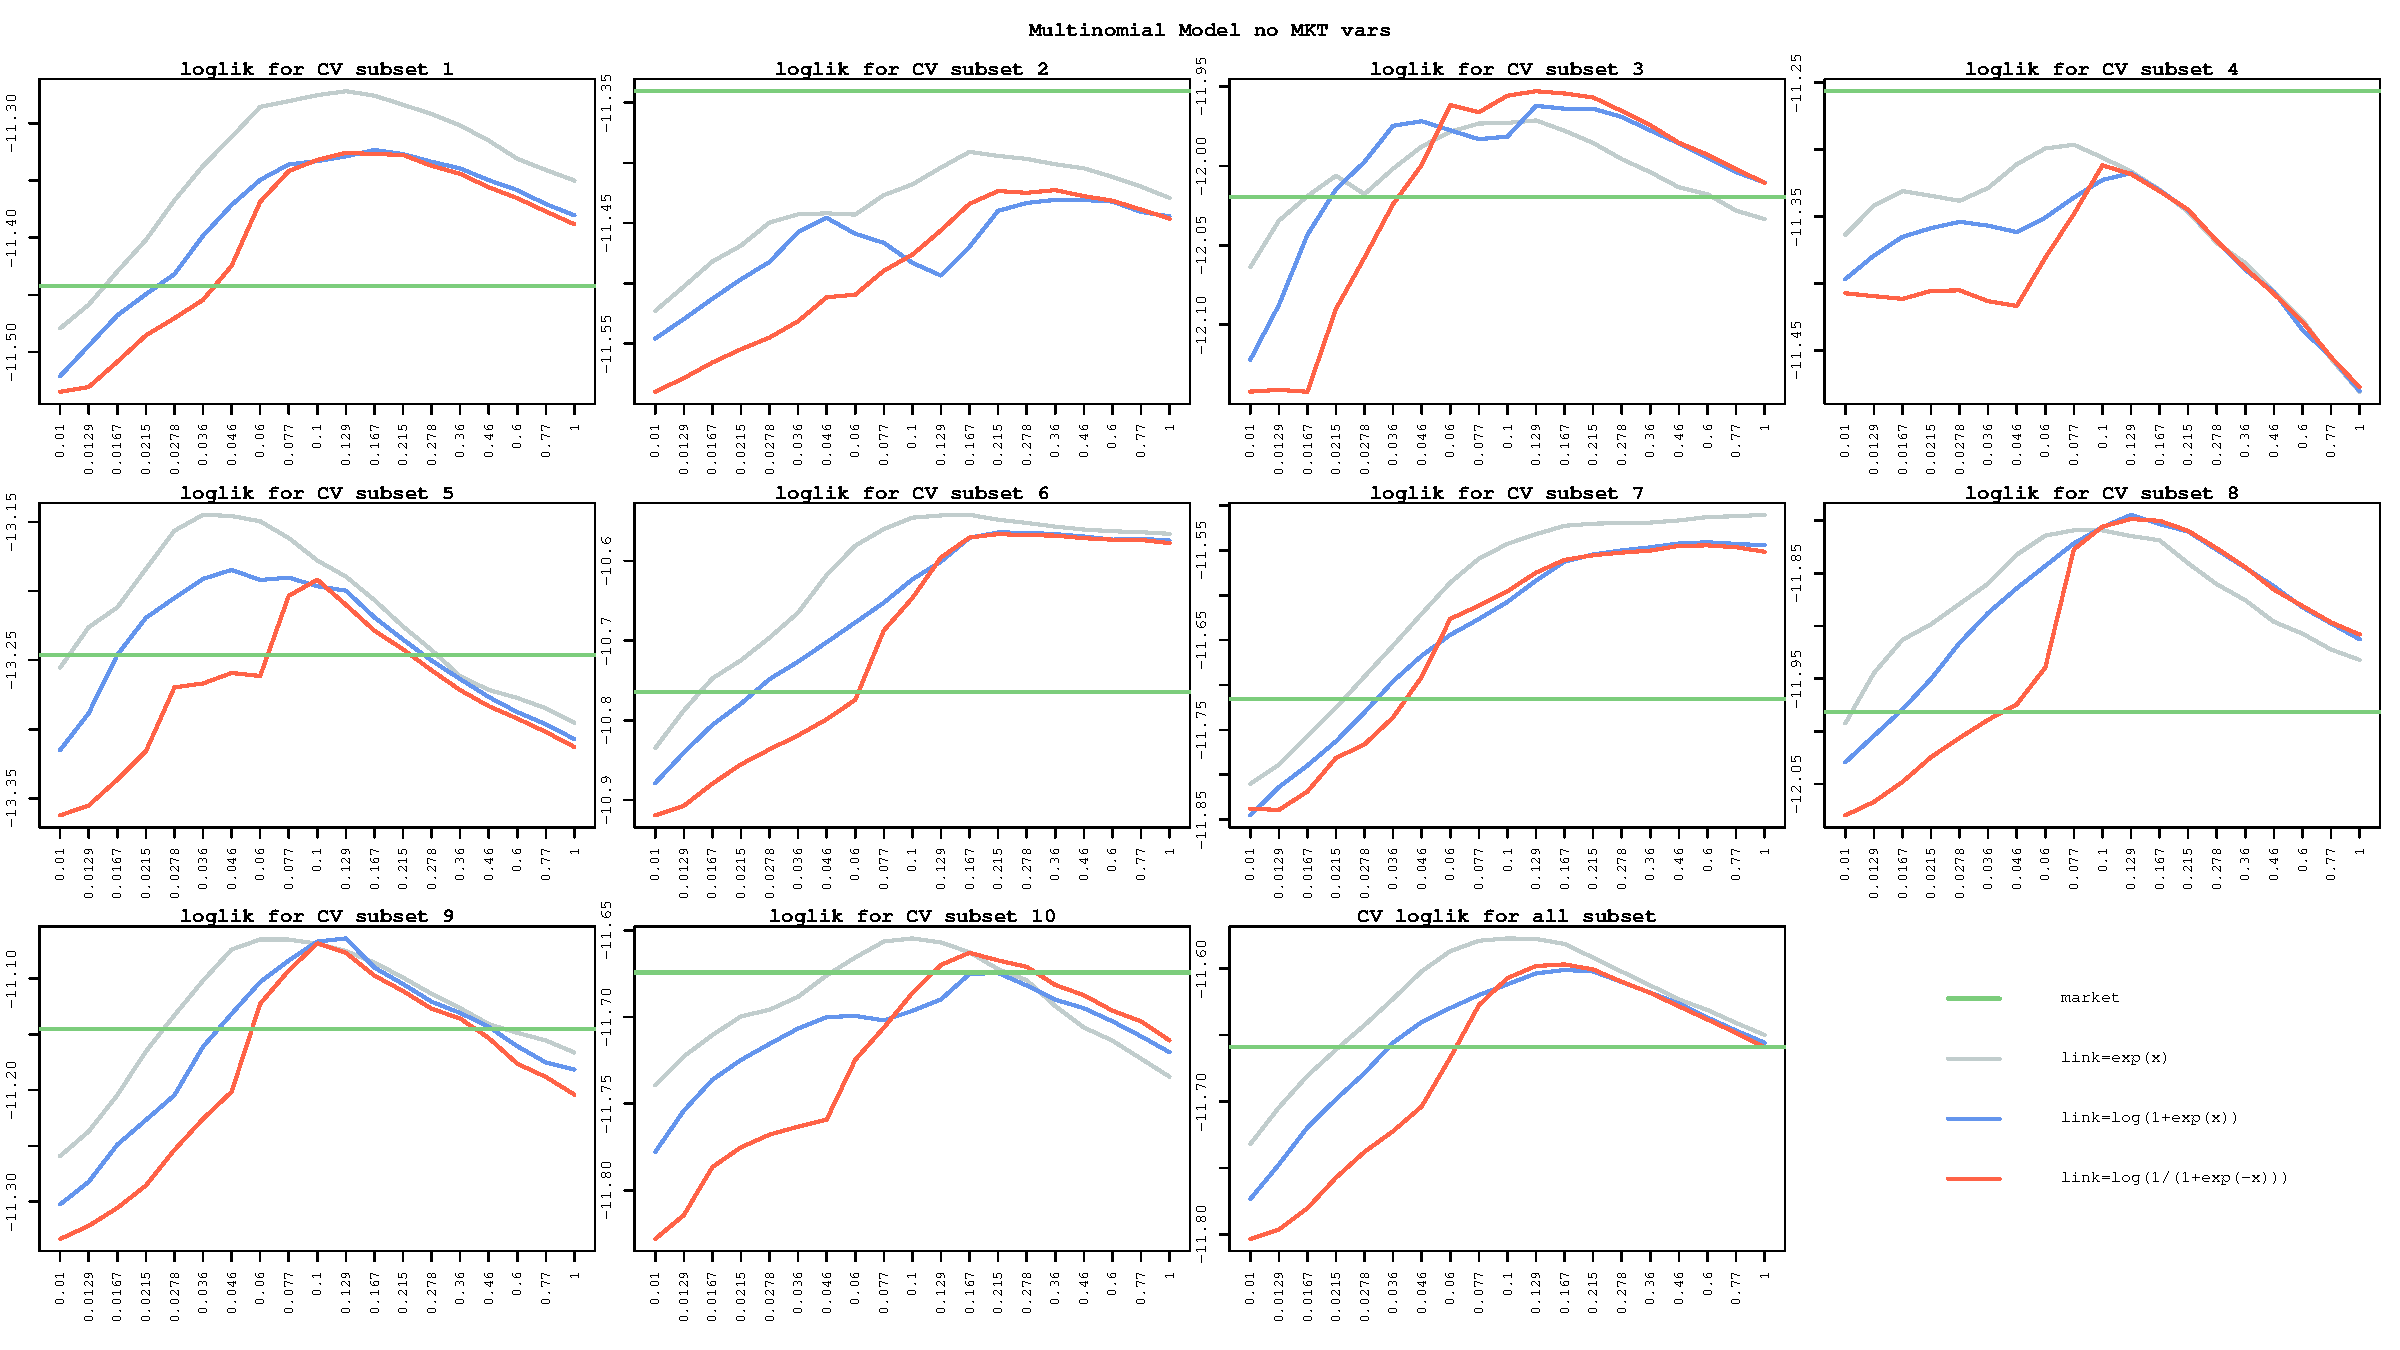
\includegraphics[width=6.5in]{compareBMNM.pdf}
%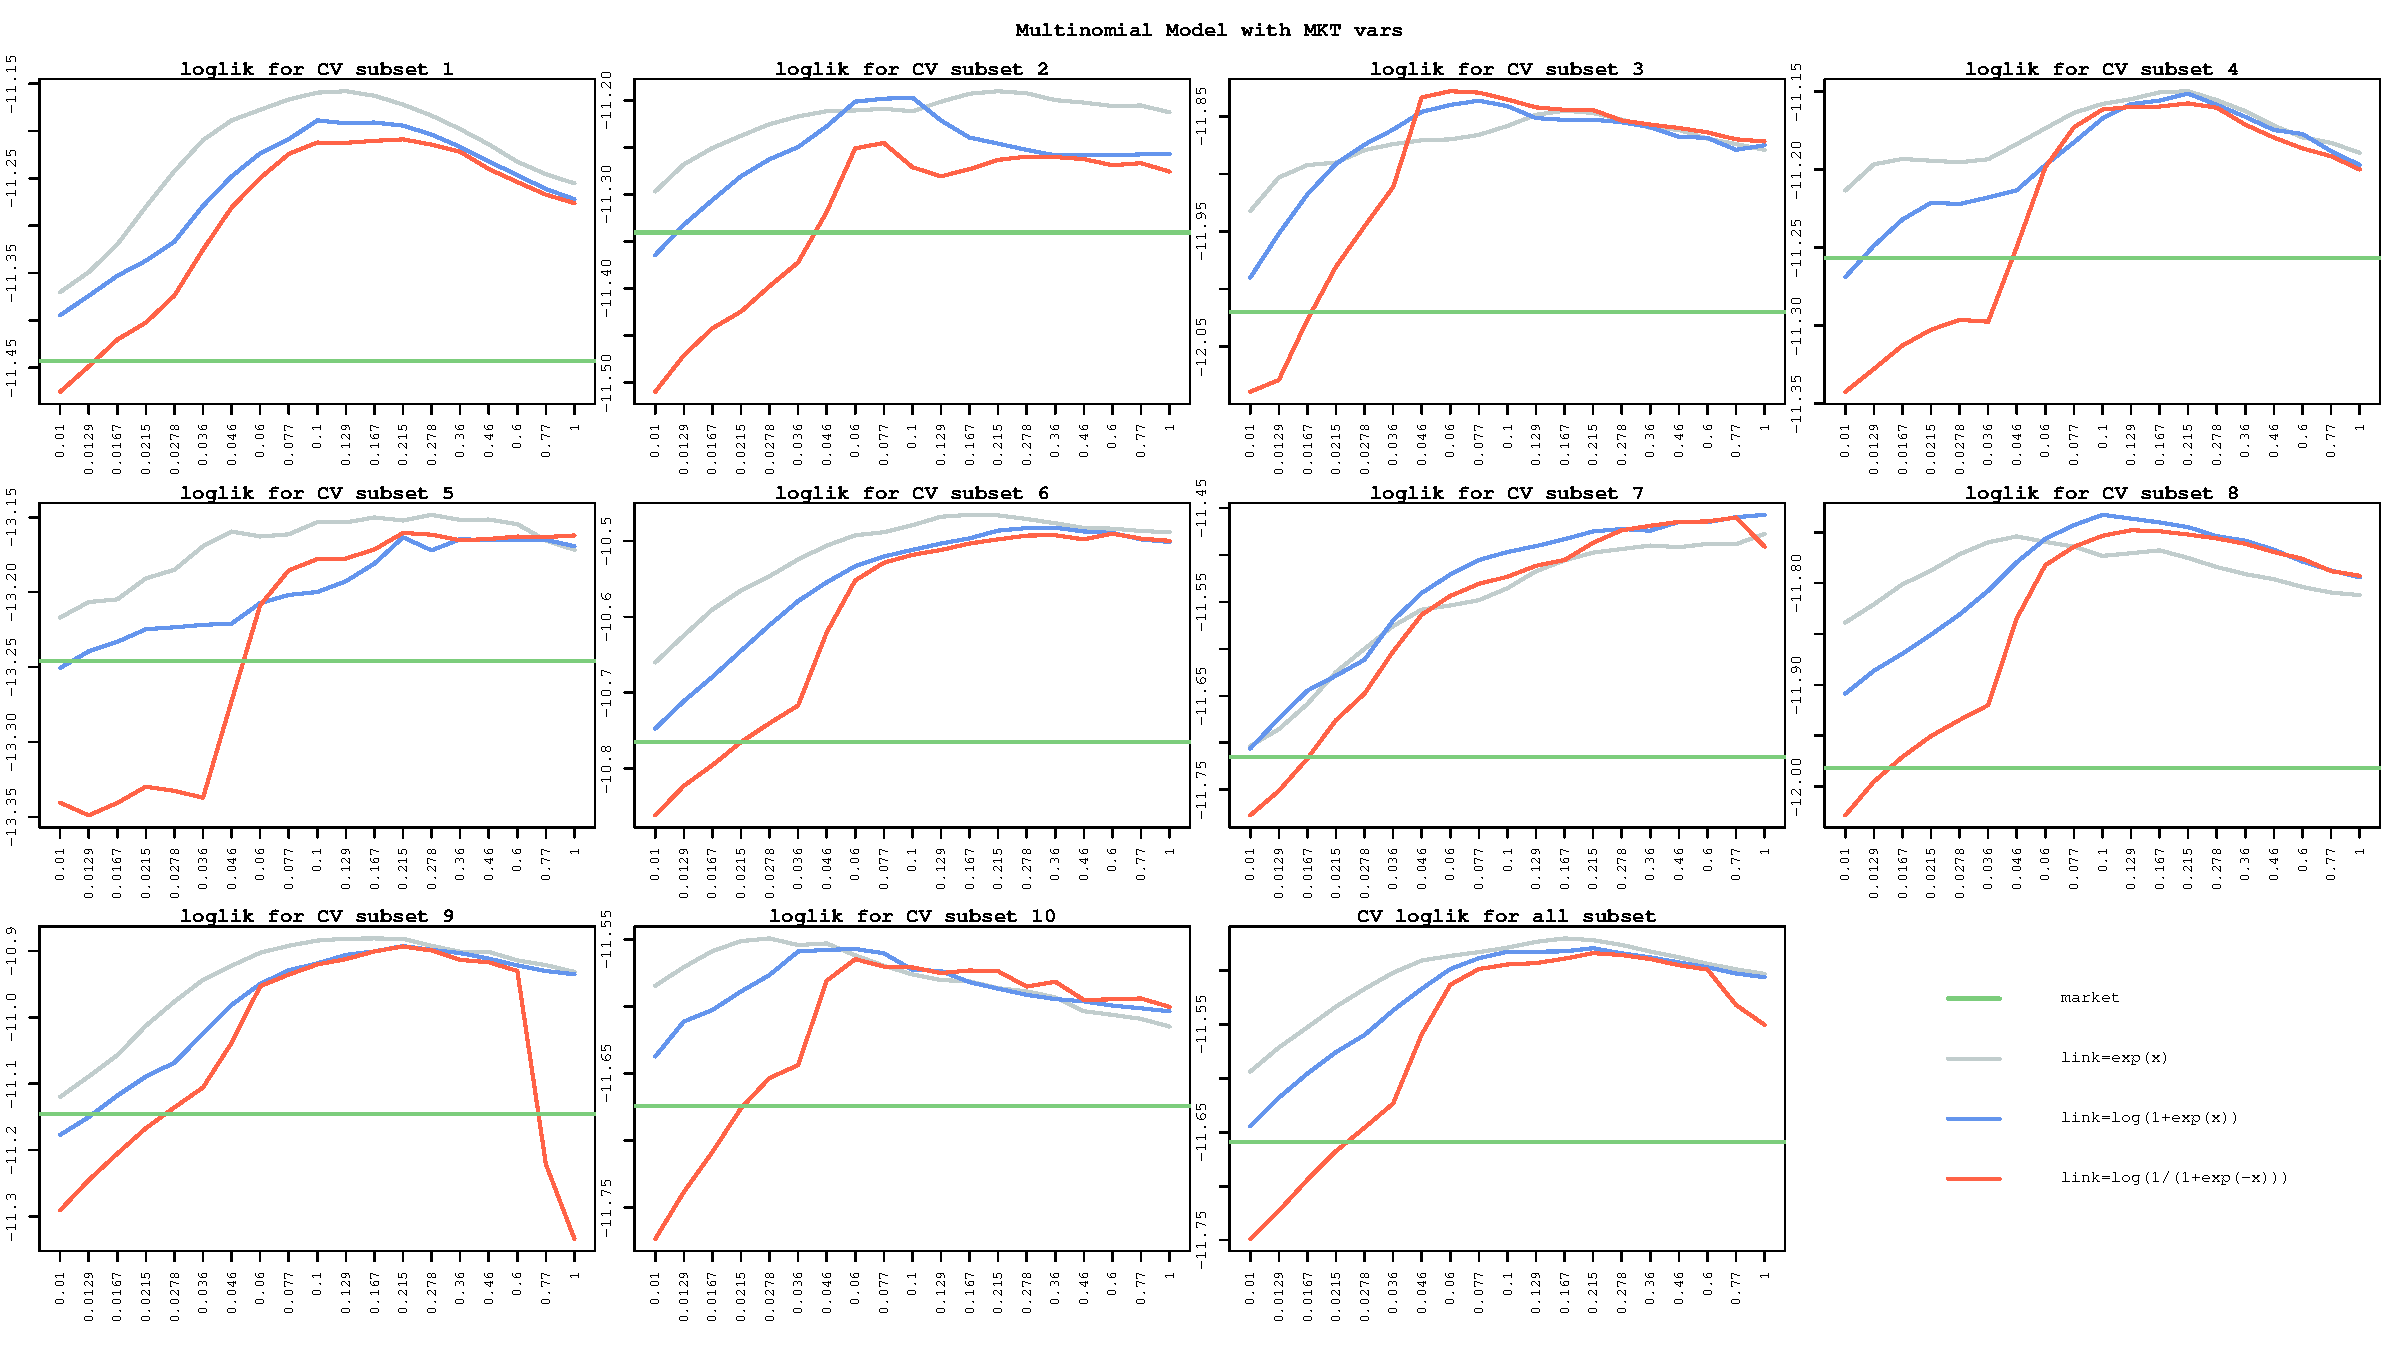
\includegraphics[width=6.5in]{compareBMWM.pdf}

\newpage
MODEL3: $y_{i.}\mid \beta, n_i,  X_{i.}\sim \mathrm{M}
    \zag{n_i, \zagv{\frac{\lambda_{id}}{\sum_{d^\star}\lambda_{id^\star}}}_{d=1}^D}$

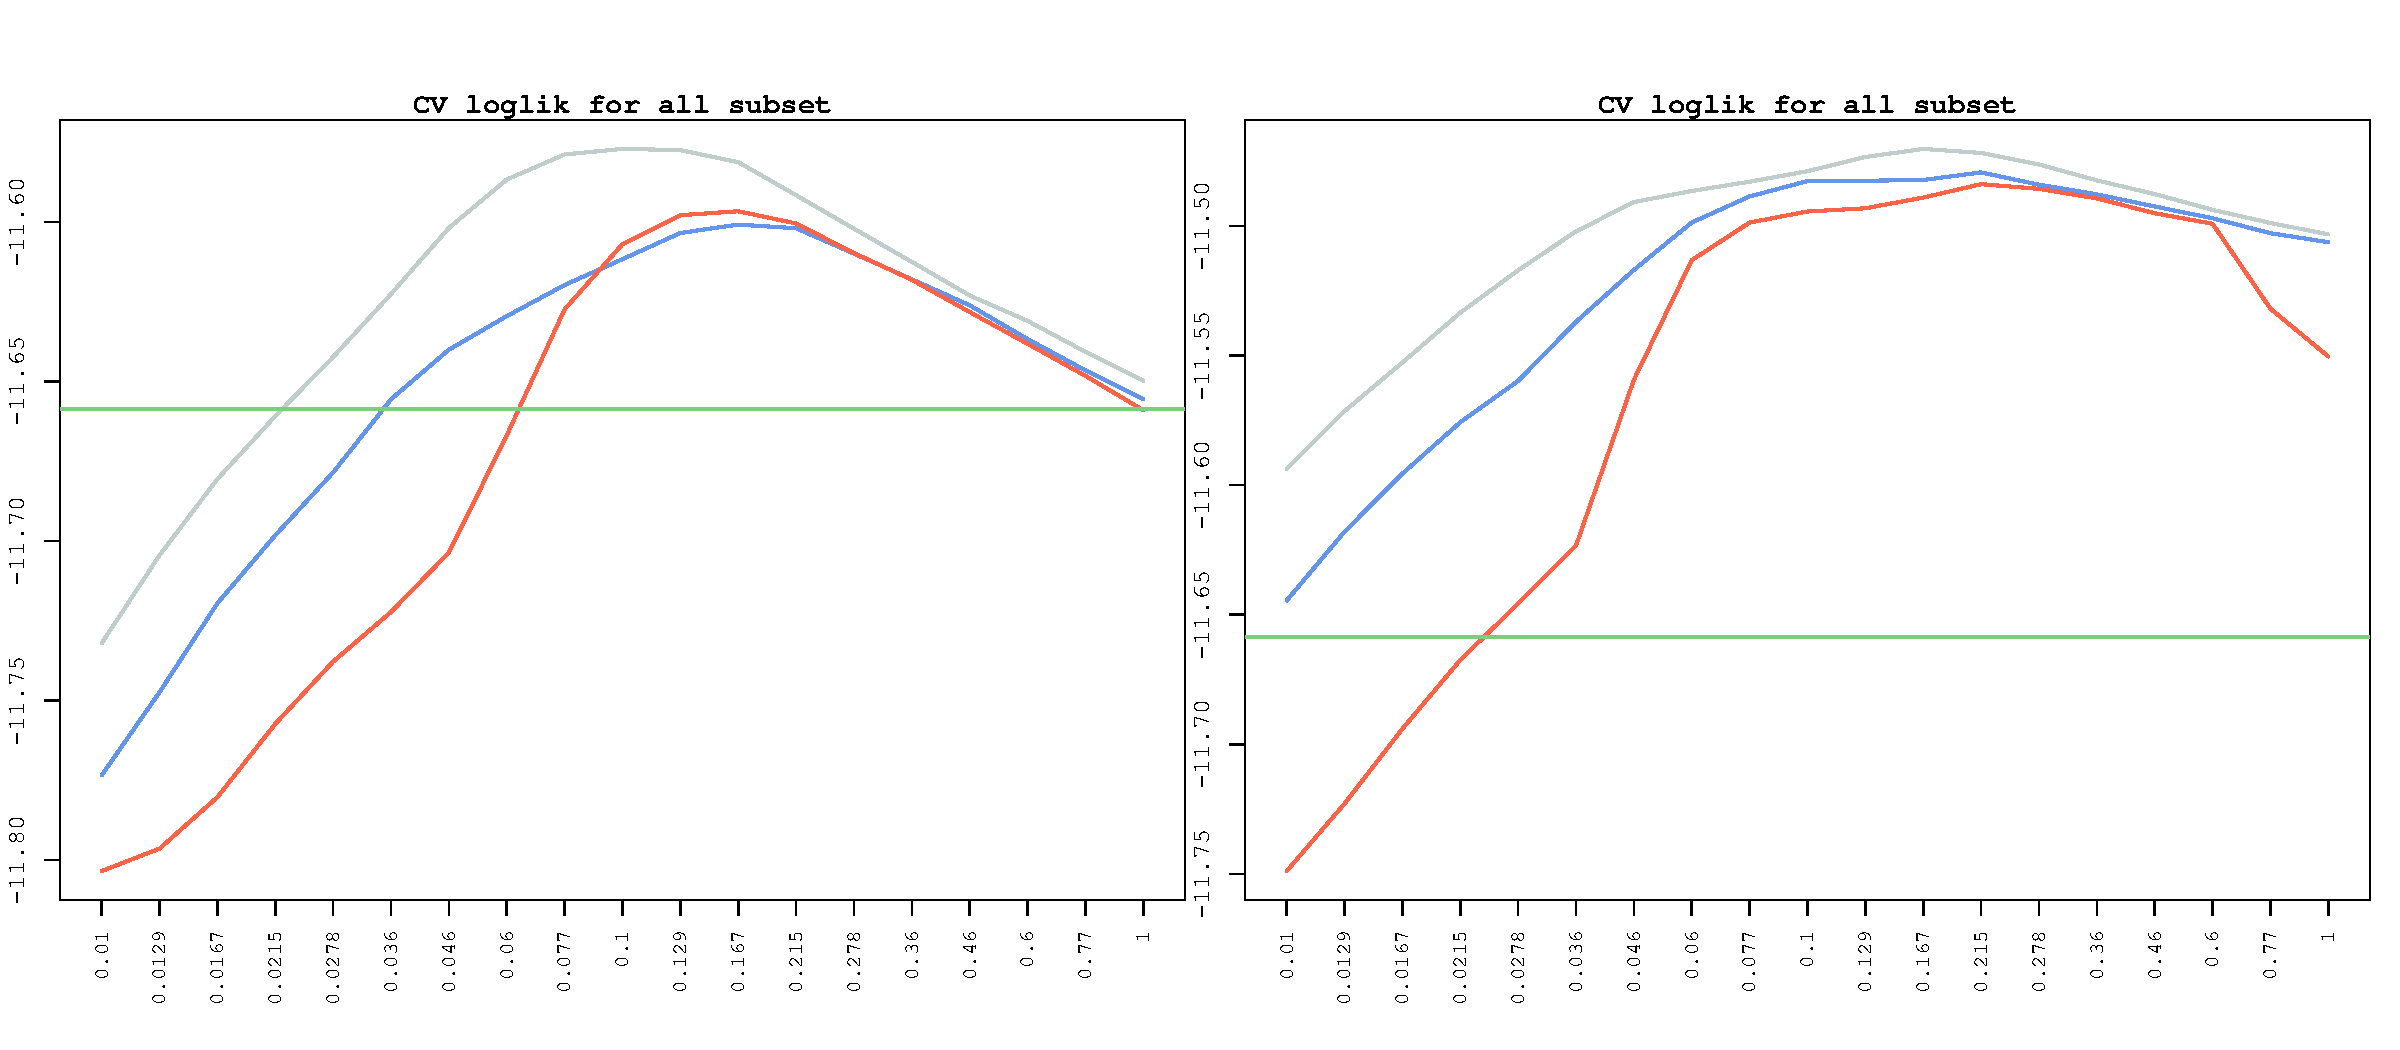
\includegraphics[width=6.5in]{MULT.pdf}

%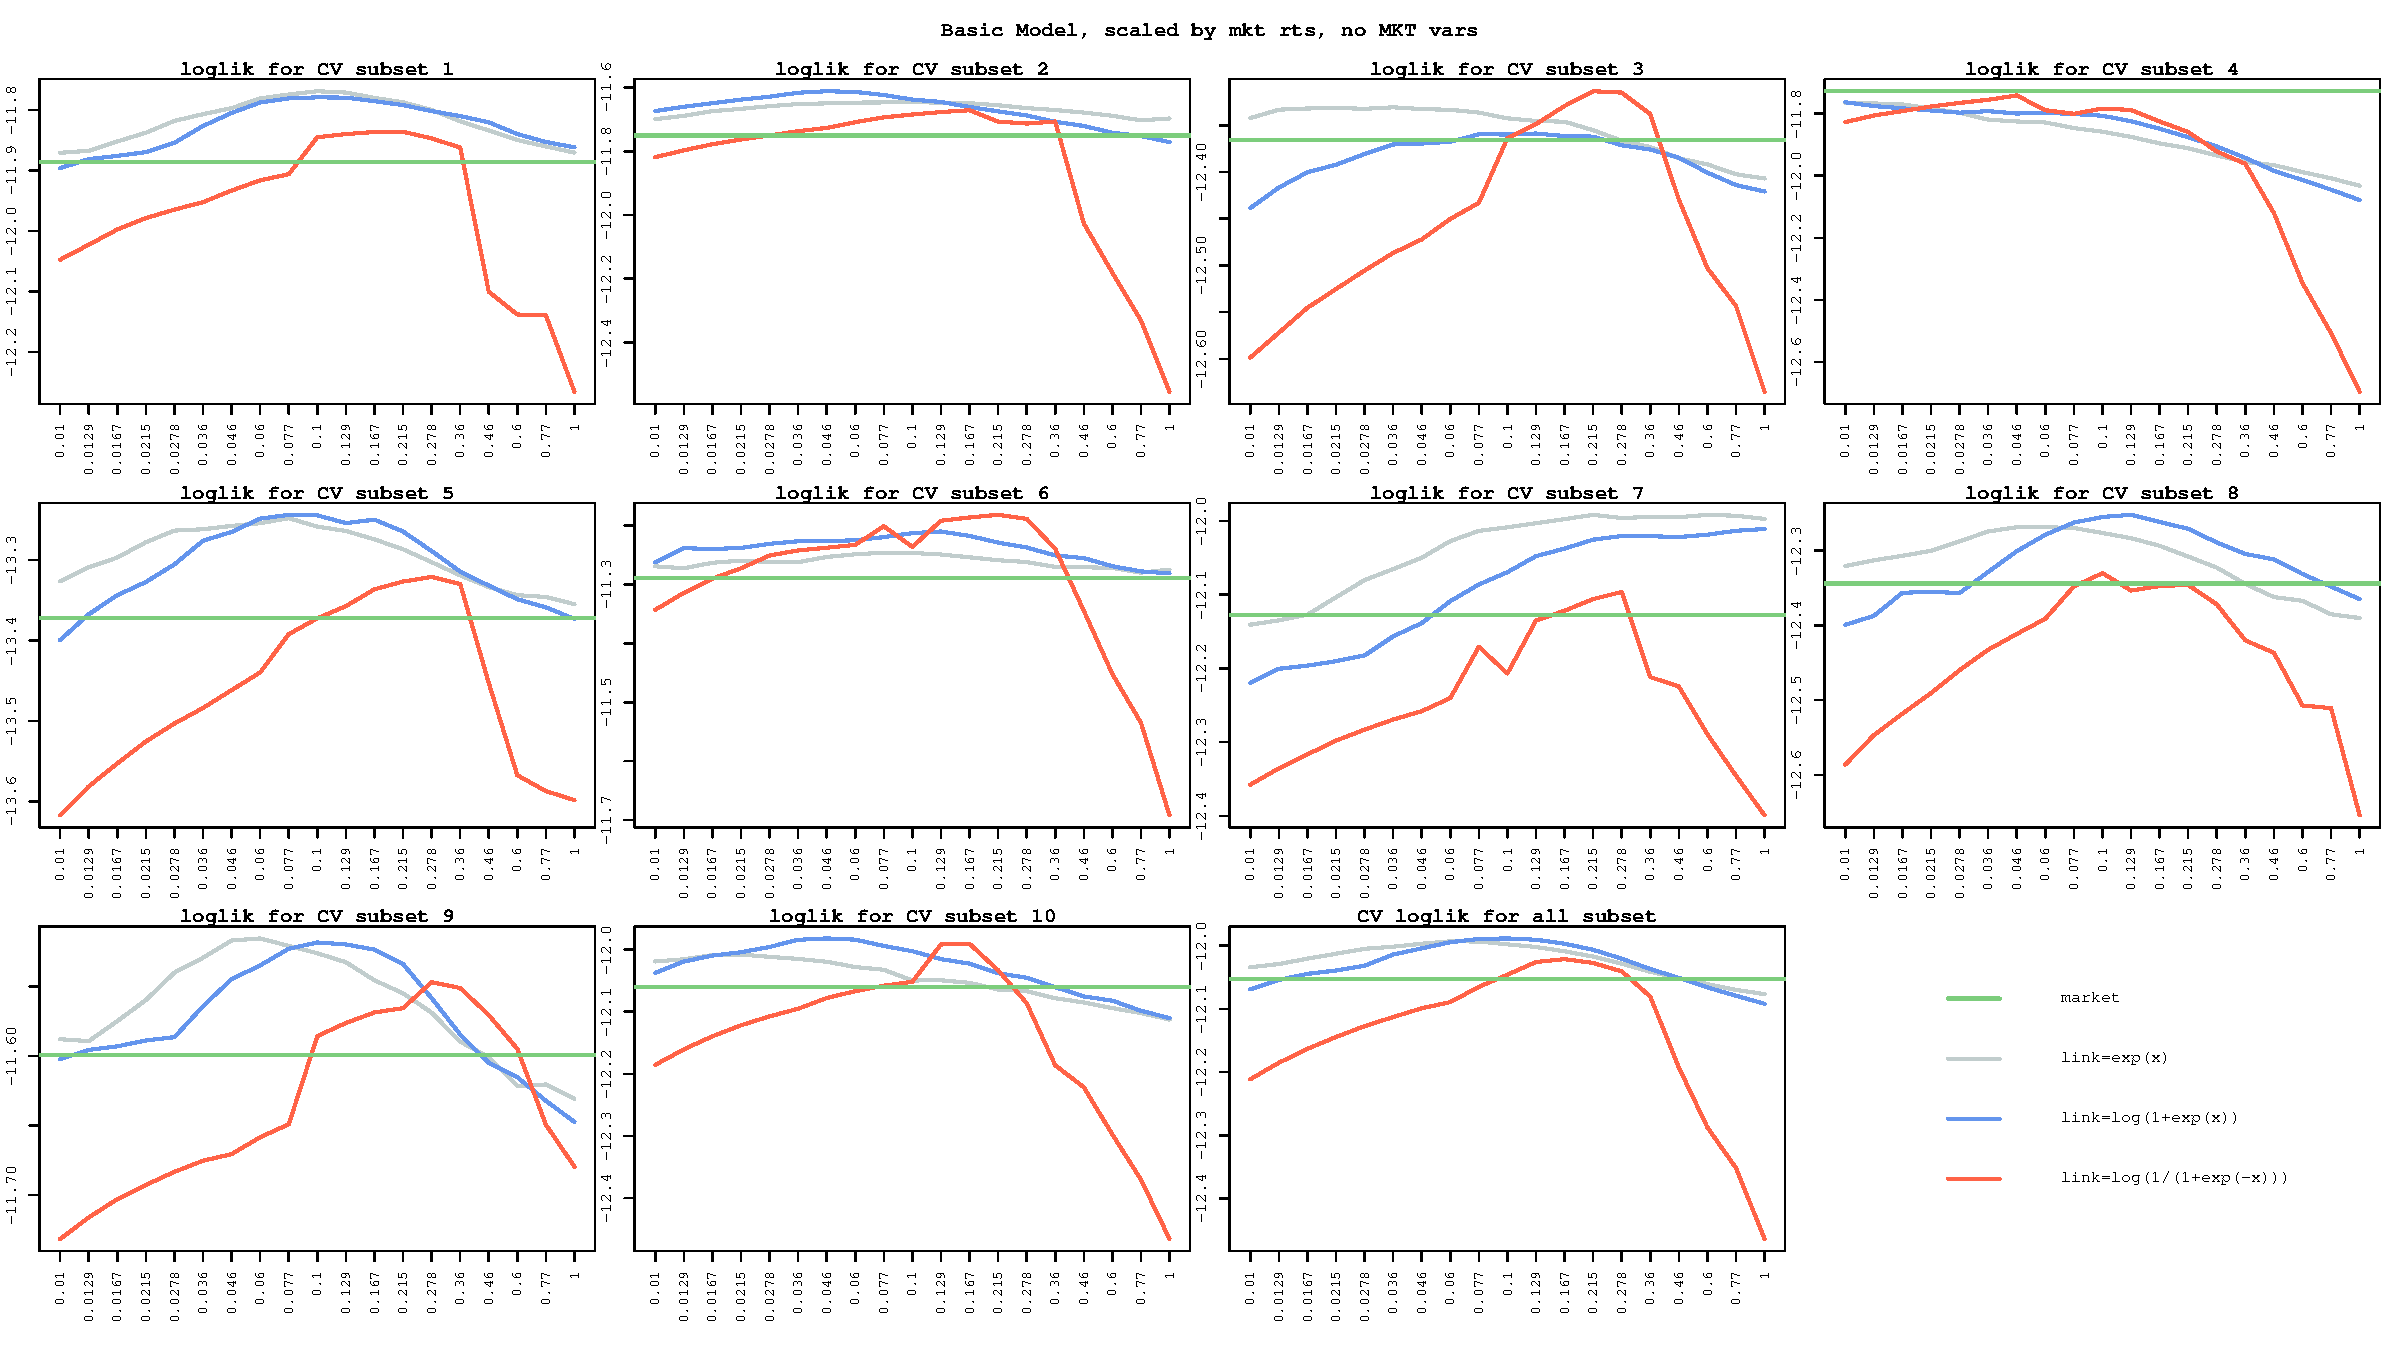
\includegraphics[width=6.5in]{compareMNM.pdf}
%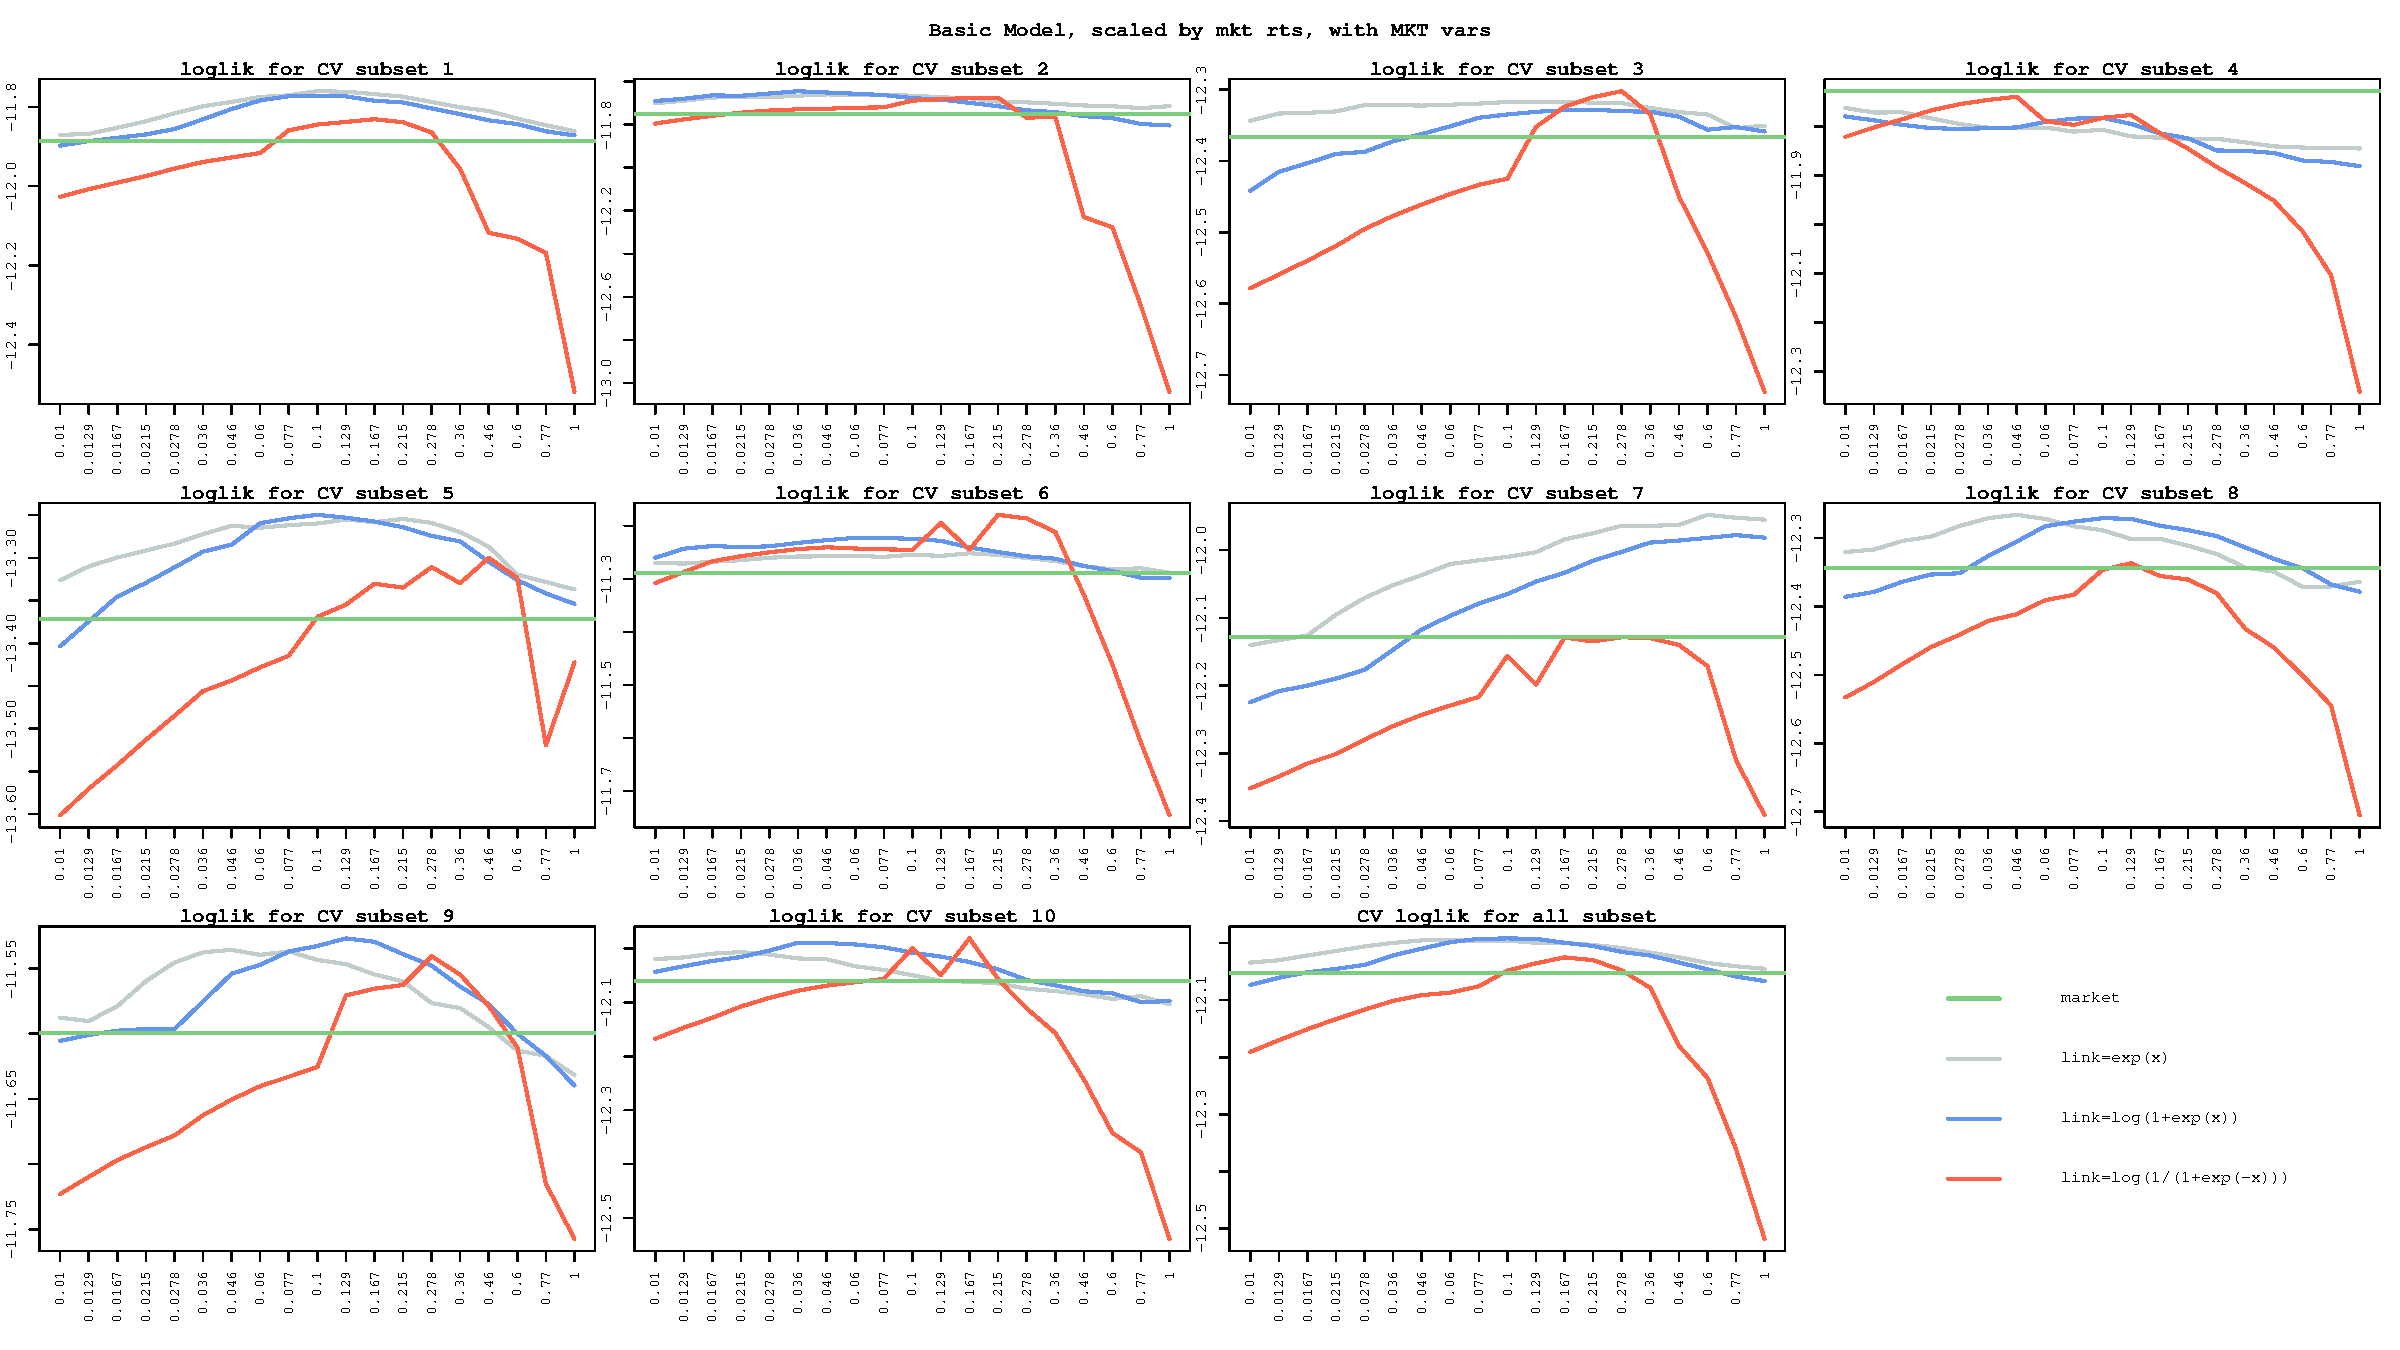
\includegraphics[width=6.5in]{compareMWM.pdf}
%\includegraphics[width=6.5in]{compareMM.pdf}

\newpage

{\LARGE INTRODUCTION: BASIC MODEL}

$$y_{id}\mid X_{id}, \beta \sim \mathrm{Pois}\zag{g(\beta^T X_{id})}$$

$$\mathrm{P}(\beta\mid X, \mathrm{Data}) \propto \mathrm{P}(\beta) \prod_i \prod_d
    g(\beta^T X_{id})^{y_{id}} e^{-g(\beta^T X_{id})}/y_{id}!$$

   -- $d$ are minutes in a match (1-44, 46-89 for both teams; D = 176 per match)\\
   -- $i$ are matches ($I=302$)\\
   -- $g$ is a link function ($\exp(x)$ is default)\\
   -- $K$ number of variables (length of beta)

$$\ell(\beta) = \log(\mathrm{P(\beta)}) + \sum_{l=(i,d)} \zags{y_l\log\zag{g(\beta^T X_l)} - g(\beta^T X_l)} + \mathrm{const}$$

is it convex with respect to beta and lambda???

In coordinatewise gradient descent algorithm in each step $k \in 1,\dots K$ we are maximizing $\ell$ as a function of one parameter $z=\beta_k$. It is fine for convex functions.

So goal is to minimize
$$h(z) = \sum_l \zags{g(r_l + (z-\beta_k)x_{lk}) - y_l\log\zag{g(r_l + (z-\beta_k)x_{lk})}} + z^2/2\tau$$

where $r_l = \beta^T X_l$ and $\tau$ is regularization parameter.

One good way to find the maximum of $\ell$ [David's paper, at al.] is that in each step we find maximum of 2nd degree Tailor polynomial of $h$, so suggested shift for $\beta_k$ will be $\Delta u_k = -h'(\beta_k)/h''(\beta_k)$ where

$$h'(\beta_k) = \sum_l \zags{g'(r_l)x_{lk} - y_l x_{lk} g'(r_l)/g(r_l)} + \beta_k/\tau$$
$$h''(\beta_k) = \sum_l \zags{g''(r_l)x_{lk}^2 - y_l x_{lk}^2 \frac{g''(r_l)g(r_l) - g'(r_l)^2}{g(r_l)^2}} + 1/\tau$$


\newpage
{\LARGE SHAWN'S MODEL}

Pros and cons


$$y_{id}\mid X_{id}, \beta \sim \mathrm{Pois}\zag{\alpha_i g(\beta^T X_{id})}$$

$$P(\beta\mid X, \mathrm{Data}) \propto P(\beta) \prod_i \prod_d
    \zag{\alpha_i g(\beta^T X_{id})}^{y_{id}} e^{-\alpha_i g(\beta^T X_{id})}/y_{id}!$$

Since $n_i = \sum_d y_{id}$ is sufficient statistic for $\alpha_i$ we should maximize

$$P(\beta\mid X, \mathrm{Data}, n) = P(\beta) \prod_i \prod_d
    \zag{\frac{g(\beta^T X_{id})}{\sum_{d^\star}g(\beta^T X_{id^\star})}}^{y_{id}}$$


$$\ell(\beta) = \log(\mathrm{P(\beta)}) + \sum_i \sum_d y_{id}\log{g(\beta^T X_{id})} -
    \sum_i n_i \log {\TS\sum_{d^\star}{g(\beta^T X_{id^\star})}} + \mathrm{const}$$

$$h(z) = \sum_i n_i \log {\TS\sum_{d}{g(r_{id} + (z-\beta_k) x_{idk})}} -
    \sum_{i,d} y_{id}\log{g(r_{id} + (z-\beta_k) x_{idk})} + z^2/2\tau$$

$$h'(\beta_k) = \sum_i n_i \frac{\sum_{d}g'(r_{id})x_{idk}}{\sum_{d} g(r_{id})} -
    \sum_{i,d} y_{id}\frac{g'(r_{id})x_{idk}}{ g(r_{id})} + \beta_k/\tau$$

\begin{equation*}
\begin{split}
h''(\beta_k) = \sum_i n_i& \frac{\zag{\sum_{d}g''(r_{id})x_{idk}^2}\zag{\sum_{d}g(r_{id})} - \zag{\sum_{d}g'(r_{id})x_{idk}}^2 }{\zag{\sum_{d} g(r_{id})}^2} \\ -&
\sum_{i,d} y_{id}x_{idk}^2\frac{g''(r_{id})g(r_{id})- {g'(r_{id})}^2}{{g(r_{id})}^2} + 1/\tau
\end{split}
\end{equation*}

\input{genetic.tex}


\end{document}


\newpage


%\input{relatedwork.tex}

METHODS:

VARIABLE SELECTION:

ALGORITHM:
Explain algorithm like David did (formulas for flexible allowed jump)

Pre-selection of good variables:


DATA:

1. Simulate fake data

2. save data in .Rdata. SoccerSmall1, SoccerSmall2, SoccerLarge1, ..., with or without interactions (double or triple)

3. First 104 variable into txt file and zip and it should  unpack and work

4. prepare different OKs


Fitters:

1. Gradient descent
2. Gradient descent for L1 with flexible allowed jumps (should include part that jumps only if it increases LL)
1. Davids like
2. Mine 1 (fix tau thing -- divide by nvar)
3. Mine 2
4. variable tau fit for forward selection (
fix tau, find best var, fix vars and find best tau, fix tau and find next best var,...)

early stopping of a fitter:

1. if adding new var doesn't improve LL.TE then it is out

2. should record the evolution of the quality of variables, to see if any becomes more important eventually.

EXPERIMENTS:

CODE:

save all interesting output of the fitter into files (condor)

write it to be more clean, prepares and saves data and results automatically (in DAG),

also load data,

loads link functions

maybe:

- have new staring point for beta

- include different tau for for fitter. Finding optimal tau?


RESULTS:

table(L2 basic, L1 basic, L2 Shawn, L1 Shawn, L2 preselected, ..., \\
TR.fit\\
TE.fit\\
time)

1. What is the result of homogenous Poisson (baseline)
2. Can we do better than market
3. Get and plot results from J0 folder. Save into .Rdata
4. for those 20000 fittings find the distributions of non-zero and of zero coefficients. Find (some) score for variables. Make a top list of variables for each tau. Is it different
5.


Picture:

How to check for significance

Saturated link does better?

PDF file for estimates


DISCUSSION:




\begin{itemize}
\item What if you add vars with largest contribution first. Best variables by forward selection could be masked. For example if we add first best then adding next two best variables one-by-one can produce worse results than finding two best at the same time.

\item When adding new best variable optimal $\tau$ can change. What is the best tau as a function of the number of parameters. Probably will be different for L1 and L2. It is decreasing as function of parameters, probably $1/n$ or $1/\sqrt{n}$

\end{itemize}










\end{document}

